\section*{Assignment 09: Scaling Strategy}
\addcontentsline{toc}{section}{Assignment 09: Scaling Strategy}

SkillSync scales in three stages. Phase one tackles product-market fit: fortify the core, test network effects within one geographic cluster, and land two local anchor partners (trade association plus municipal innovation unit) so their signalling power lifts both sides at once \citep{Choudary2016,Reillier2017}. We keep a focused growth pod, two developers for stability, and a community manager shepherding feedback loops in the pilot Slack.

Phase two covers regional scaling. We standardise onboarding flows and API contracts so partners plug in without hand-holding, run a three-tier programme (community, certified, strategic) to manage quality and incentives \citep{HagiuWright2013}, staff a lean partner-success team, ship shared dashboards, and track cross-side conversion plus time-to-value per partner to see whether network effects accelerate \citep{ShapiroVarian1999,Lecture12}.

\begin{figure}[h]
  \centering
  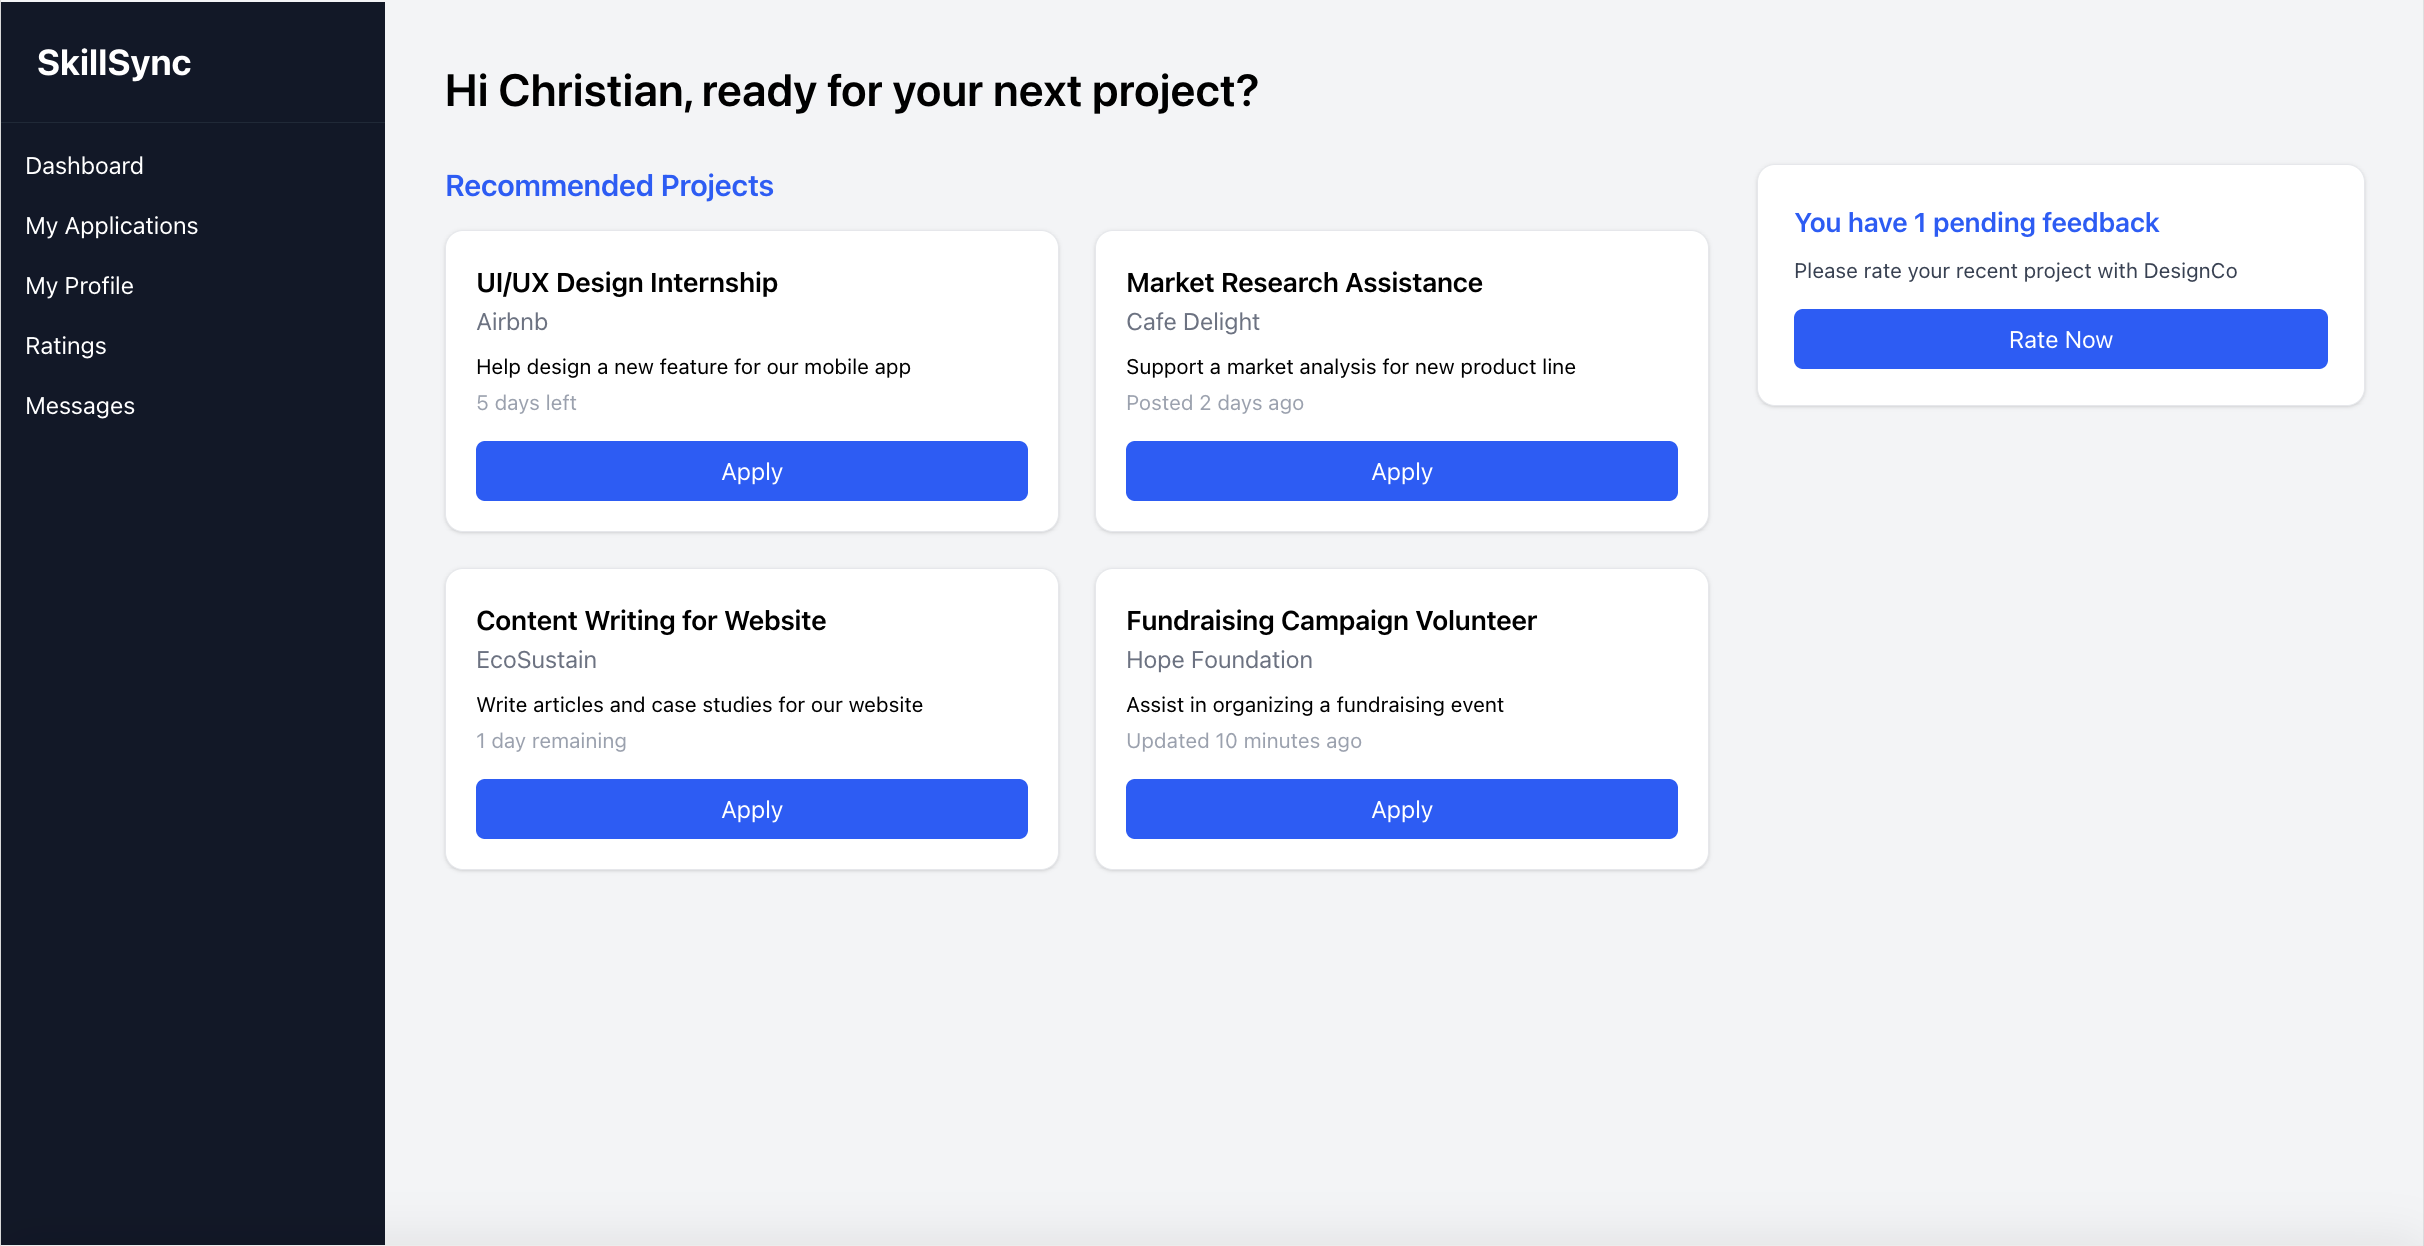
\includegraphics[width=0.75\linewidth]{Student-Dashboard.png}
  \caption{Adoption dashboard (`Student-Dashboard.png`).}
  \label{fig:scaling-dashboard}
\end{figure}

Figure~\ref{fig:scaling-dashboard} (based on `Student-Dashboard.png`) keeps the SkillSync crew honest by showing how activation rates inflect only after partner enablement becomes self-serve, so we resist the temptation to sprint ahead until the curve bends.

Phase three moves national (maybe Nordic) once the first two phases prove unit economics. We court alliances with larger institutional players, negotiate white-label deals with select enterprise clients, and expand governance with clear data-sharing principles, algorithm audits, and an advisory board so legitimacy scales \citep{Srnicek2017,Zuboff2019}. Budget also covers compliance expertise, localisation, and a small deal desk that can tailor partnerships without wrecking the standard product.

Two risks dominate: churn and quality decay. Churn can hit users or partners, especially if competitors tempt them with exclusive features or lower fees, so we build switching costs through data portability, loyalty loops, and analytics that lose value if someone leaves \citep{FarrellSaloner1986,ShapiroVarian1999}. Quality decay flares when growth dilutes standards, so we enforce service-level agreements, automate match-quality monitoring, and run quarterly partner reviews with a community board catching soft signals before the dashboards scream \citep{Reillier2017}.

Theory lines up with the platform canon: network effects need critical mass but pushing too fast erodes match quality and differentiation \citep{Porter2008}. \citet{Choudary2016} remind us governance and producer enablement must evolve with each phase, while \citet{Srnicek2017} stresses pairing aggressive growth with legitimacy and transparency, so we keep investing in partnerships and organisational scaffolding.

We stress-tested the roadmap with a simple Google Sheets simulation covering activation rate, partner velocity, moderation load, and average project value. It tells us how many moderators and partner managers we need per 1,000 active users, how big a churn buffer to hold, and when to pause expansion: if quality drops below 4.4/5 for two months we freeze new partners until the governance board approves remediation, feeding the admin panel from Assignment~05.

To keep scaling humane we end each phase with a ``story harvest'' where students, NGOs, and team members share surprises. The stories feed marketing assets, internal training, and quarterly retros using \citet{Choudary2016}'s interaction-model canvas so the platform stays a living system.
